\section{Integration}

\subsection{Overview}

This section describes the process of integrating the trained surrogate model into the MEDEAS model.

The MEDEAS model is built with the \href{https://vensim.com/}{Vensim} software, and is available to the public as a Vensim model file. However, the python library \href{https://pysd.readthedocs.io/en/master/index.html}{\texttt{pysd}} \cite{pysd}, focused on system dynamics simulations, is able to parse such files and run the simulations. The reasons why this will not be taken advantage of is discussed in the first subsection.

The task of integrating the surrogate model into MEDEAS is split in two smaller steps:
\begin{enumerate}
    \item \textbf{Vensim integration}, that is to make the surrogate model, available as a Tensorflow model, callable from within a Vensim model
    \item \textbf{Variable linking}, Link the input and output features of the surrogate model to the actual variables used in the MEDEAS model
\end{enumerate}

\subsection{Vensim integration}

\subsubsection{The Vensim software}

\href{https://vensim.com/}{Vensim} is a system dynamics simulation software, developped by Ventana Systems, Inc. It primarily solves the system of differential equation represented by the user-defined model, and is mainly used, according to its description, "for developing, analyzing, and packaging dynamic feedback models" \cite{vensim-website}.

Its most common application areas include \cite{wiki-vensim}:
\begin{itemize}
    \item Transportation and energy,
    \item Project management,
    \item Environment.
\end{itemize}

Vensim also comes in different distribution, such as Vensim PLE that is the free, personal learning edition. In this work, Vensim DSS is used, with an academic license.


\subsubsection{Vensim models}

Vensim provides a variety of tools to describe models, but at the end every model is an interconnection of variables, the math hiding in the connections between these. 

Vensim provides the following types of variables:
\begin{itemize}
    \item \textbf{Auxiliary variables}, that are regular variable that have no memory, that is, are independent from their value at the previous time step and are computed from every type of variable.

    For example, a $temperature$ variable that is computed from some $sunshine$ and $latitude$, that is used to compute the birth rate of $rabbits$ and $foxes$.

    \item \textbf{Constant variables}, that hold one value.
    
    For example, a mathematical constant like $\pi$.

    \item \textbf{Data variables}, or exogenous variables, whose value evolve over time but is not dependent of the model.

    For example, typical $sunshine$ data over a year.

    \item \textbf{Stock variables}, that change only over time as a function of the incoming rates, i.e., they integrates the rates.

    For example, the population of some species at a given time.

    \item \textbf{Rate variables}, or flows, that directly impact the Stock variables. 

    For example, the birth or death rate of some population at a given time.
\end{itemize}

The connections between the variables are virtually done by arrows. The only practical use of arrows is to make the variable at the origin appear in the selection of variables in the variable equation screen for the variable pointed by the arrow. But obviously they are of great utility in terms of visualization of the model.

An example of a Vensim model is depicted in Figure \ref{fig:vensim-model-example}.

\begin{figure}[h!]
    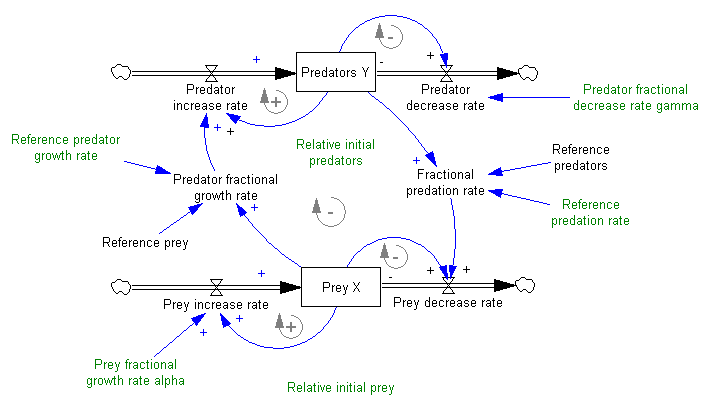
\includegraphics[width=0.9\textwidth]{resources/images/vensim-model-example.png}
    \caption{An example model in Vensim: Lotka-Volterra predator-prey model.}
    \label{fig:vensim-model-example}
\end{figure}

\subsubsection{Vensim external functions}

This specific feature of the Vensim software is evidently of great interest for this work. It enables the user to provide and use any arbitrary function in Vensim models and simulations.

To do so, the user needs to provide a dynamically linked library (DLL), packaged as a \texttt{dll} file, then provide its path in Vensim. These files are Windows specific (as Linux uses \texttt{so} files and macOS \texttt{dylib}), hence they have to be handled as such.

Dynamically linked libraries are pieces of compiled code that can be loaded at runtime by another program. User-defined functions necessarily need to be loaded at runtime, as the software cannot know them in advance. These are typically compiled from the C or C++ programming language. In this work, C++ has been chosen, as the library to load and call Tensorflow models that will be used is written in that language.

To be able to integrate the user-defined functions in its simulation environment, the user's library is expected to provide some functions, that are part of some interface that the Vensim software knows and can communicate with. This interface comprises of a set of functions that is described in Table \ref{table:vensim-interface}.
\begin{table}[h]
    \centering
    \begin{tabular}{|m{4.1cm}|m{12cm}|}
        \hline
        Function name & Description \\ \hline
        \texttt{version\_info} & Provide information about the Vensim version this library has been built for \\
        \texttt{set\_gv} & Utility to set the global variable that depend on the Vensim simulation environment \\
        \texttt{user\_definition} & Provide a way to get all the necessary information about each user-defined function, mostly their names, number of arguments and a identifier code \\
        \texttt{simulation\_setup} & This function is called by Vensim on simulation startup, allowing the library to do some preparative work if needed, such as allocating memory \\
        \texttt{simulation\_shutdown} & Same as \texttt{simulation\_setup}, but on simulation shutdown \\
        \texttt{vensim\_external} & This function is expected to, given an array of input arguments, their number and a function code, call the function associated to that code and write its return value into the first input argument.\\
        \hline
    \end{tabular}
    \caption{Description of the mandatory functions that a Vensim user library has to provide}
    \label{table:vensim-interface}
\end{table}

Luckily, %I'm not afraid of the dark
Vensim DSS ships with an example of such a library. As this file is not publicly disclosed, caution should be paid to keeping the library code private---actually, the external function capability is only available in Vensim DSS.

In the implementation of the library, this file was copied then adapted, as suggested in Vensim's documentation.

\subsubsection{Vensim subscripts}

This feature of Vensim is advertised as one of its most powerful tools. These allow to subscript variables appearing in the equations and perform operations across subscripted values if needed. For example, it enables to set predators and preys initial populations and reproduction parameters for several environments, and run them all at once. 

Importantly, MEDEAS use subscripts to run several simulations in parallel called scenarios. Therefore, one needs to edit the subscript properties in order to manage the scenario that will be run and displayed.

\subsubsection{Calling a Tensorflow model}

In consequence, it is necessary to invoke our model, presented to as a Tensorflow model, from the C or C++ language.

In order to do so, one basically needs two things:
\begin{itemize}
    \item the model in question, saved in a directory from the Tensorflow python API.
    \item the Tensorflow library, which is another DLL, to perform the actual computations from C/C++.
\end{itemize}

The complicated part being the linking between the two. In order to do so, the \href{https://serizba.github.io/cppflow/}{Cppflow} tool is used. It serves as an intermediary layer between C++ and the Tensorflow model. This tool is not available in C, this is the primary reason why the library is implemented in C++.

The main purpose of Cppflow is precisely to run Tensorflow models from C++, and to achieve this it provides user-friendly functions for loading models and making predictions using input data.

To ensure proper linkage between the library code and the two tools it utilizes—Tensorflow DLL and CppFlow—an appropriate linking strategy is necessary. To facilitate this, Makefiles were crafted using the GNU \texttt{make} utility for streamlined compilation\footnote{Previously, a program calling a Tensorflow model was created, but this did not worked from the DLL. Then, a workaround was developed using a worker process (a seperate program) and Windows' tools for interprocess communication. Later, it was discovered that the issue with calling Tensorflow stemmed from errors in linker arguments during library compilation. Once these linker issues were resolved, the need for the worker process workaround became redundant.}.

On this, one thing is to be remembered: some code may compile and link successfully, but one also has to link properly the path to the DLL you linked to, that is, not only to the compiler.

% \subsubsection{A small detour...}

% At some time in the library developpement process, it was successfully managed to produce a standalone program loading the Tensorflow model, and calling it on some inputs, but this was not the case for the library, that was able to compile and link, but not to find the DLL, once called from Vensim.

% It has been thought it may not be possible, so a workaround was implemented.

% The idea was thus to make the library communicate with another program, that would be launched as a separate process. The library would thus start the other program as an external process, that will be waiting for computation queries, on simulation setup, and end it on simulation shutdown. Then, when the model is called from the library, it sends the input to that other process, which calls the model, and sends back the output to the library, that can return.

% As previously mentioned, DLL are specific to Windows, so the process management and inter-process commication had to be done in that context.

% \subsubsection{And a fix}

% But during some more testing, and adapting of \texttt{Makefile}s, the mistake was discovered: the compilation command used to produce the library missed the indication of the path to the DLL.

% With that fixed, the library can directly use the Cppflow utilities, what greatly simplifies its architecture and code. The simulation setup loads the model, the model calls use it, and finally the simulation shutdown routine frees it.

\subsection{The pysd option}

As previously introced, the \texttt{pysd} python library can read and run Vensim model files. Of course, as the surrogate model is primarily defined in that language, one would deduce that its integration would be easier that way.

Though not explored in this work, integrating the surrogate model through \texttt{pysd} is expected to be relatively straightforward. Using the library loading functionality, a python module representing the simulation can be obtained. This module is then loaded with \texttt{pysd} to run the simulation. The linking can thus be done by editing the module file directly, and inserting the call to the model at the appropriate place. 

However, this approach was not selected. Although contemplated later in the project, after the integration into Vensim had been implemented, the main argument is the convenience of the resulting model. If the model combination was made available sa python module, it would be much harder for external people to edit the original MEDEAS model from Vensim, then run the modified version while keeping the surrogate model integrated. The editor would have to manually re-insert the surrogate model into the python module, that also have to be recreated.

Keeping the surrogate model available as a Vensim external function is therefore a significant benefit for the further improvements of the model, as it enables edits to be made to MEDEAS independently of the surrogate model.

Another update has to be mentionned here. In facts, J. Paris had trouble making the MEDEAS model run successfully with the integrated surrogate model had contact with the MEDEAS developping team, that advised to wait for the release of a update of the MEDEAS port to python, making use of \texttt{pysd} and expected to be more stable and convenient. The main issue was that she were to leave before the anticipated release date, such that it was not acheivable.

This newer Python port with \texttt{pysd} might ultimately render direct integration in Python more portable and convenient. This would offer the same advantage as the Vensim external function. Still, this function was created and finished before learning the future availability of the new python port.

\subsection{Variable linking}

In its underlying workings, the MEDEAS model does not directly employ all the variables that appear in our surrogate model. This necessitates establishing connections between the two.

Fortunately, many of the desired values bear a close relationship to existing variables within the MEDEAS energy module, so these links are expected to be as simple as linear rescalings or combinations.

The input variables, that are summarized in Table \ref{table:reference-values}, do not map directly to already existing variables in the MEDEAS model. Thus, some mappings have to be made between the inputs and outputs of the surrogate model, the Dispa-SET side, and the MEDEAS side.

This work has been done with the help of Jade Paris, a student making her master's stage thesis on this specific topic as well.

\subsubsection{Variables available in MEDEAS}

The first step in this process is to list relevant variable present in MEDEAS, that will have to be exploited in order to draw the connections.

These variable are listed in Table \ref{tab:medeas-vars}.

\begin{table}[h]
    \centering
    \begin{tabular}{|p{5cm}|p{5cm}|p{1cm}|p{4cm}|} \hline 
    MEDEAS variable name &  Description & Unit & Notation \\ \hline
     FE elec generation from solar PV TWh & Total yearly production from solar photovoltaic units & TWh & $Generation_{PV}$\\ \hline 
     Total FE Elec demand TWh & Yearly total electricity demand & TWh & $Demand_{tot}$ \\ \hline 
     FE Elec generation from offshore wind TWh & Total yearly production from offshore wind turbines & TWh & $Generation_{wind-offshore}$ \\ \hline 
     FE Elec generation from onshore wind TWh & Total yearly production from onshore wind turbines & TWh & $Generation_{wind-onshore}$ \\ \hline 
     Total capacity elec storage TW & Total power output of storage units & TW & $Storage_{tot}$ \\ \hline 
     Total FE Elec genetaion TWh EU & Total yearly electricity production from all units & TWh & $Generation_{tot}$ \\ \hline 
     new capacity installed growth rate RES elec & Yearly growth rate of the electric network capacity & [$\cdot$] & $Growth_{capacity}$ \\ \hline
    \end{tabular}
    \caption{Relevant variable in MEDEAS}
    \label{tab:medeas-vars}
\end{table}

Unfortunately, some values are not present at all in MEDEAS, so that they can't be deduced from the model as is. But as these are mandatory to run the model, a value has to be provided imperatively. In this case, a constant value will be set.

These parameters have been introduced into MEDEAS, and their potential impact on the results must be evaluated. That is, as these may have an influence on the results, this influence will have to be assessed.

\subsubsection{Linkings}

The equations linking the input variables from the surrogate model to the MEDEAS variables are provided in Table \ref{tab:linking-equations}.

\begin{table}[h]
    \centering
    \begin{tabular}{|m{3.6cm}|c|}
    \hline 
    Input variable (from surrogate model) & Linking equation \\ \hline
    $share_{PV}$ & $share_{PV}=\dfrac{Generation_{PV}}{Demand_{tot}}$ \\ \hline 
    $share_{wind}$ & $share_{wind}=\dfrac{Generation_{wind-onshore} + Generation_{wind-offshore}}{Demand_{tot}}$ \\ \hline 
    $share_{flex}$ & $share_{flex}=40\%$ \\ \hline 
    $share_{storage}$ & $share_{storage}=\dfrac{Storage_{tot}}{Demand_{tot}}\times 365\times 24$ \\ \hline 
    $Capacity_{ratio}$ & $Capacity_{ratio}=\dfrac{Generation_{tot}}{Demand_{tot}}$ \\ \hline 
    $rNTC$ & $rNTC= Growth_{capacity}$ \\ \hline 
    \end{tabular}
    \caption{Variable linking equations. The left-hand side are Dispa-SET variables, and right-hand side MEDEAS variables.}
    \label{tab:linking-equations}
\end{table}

These connections must be implemented within the Vensim model, or incorporated directly into the computation when utilizing the python version of MEDEAS.